
%% bare_conf.tex
%% V1.3
%% 2007/01/11
%% by Michael Shell
%% See:
%% http://www.michaelshell.org/
%% for current contact information.
%%
%% This is a skeleton file demonstrating the use of IEEEtran.cls
%% (requires IEEEtran.cls version 1.7 or later) with an IEEE conference paper.
%%
%% Support sites:
%% http://www.michaelshell.org/tex/ieeetran/
%% http://www.ctan.org/tex-archive/macros/latex/contrib/IEEEtran/
%% and
%% http://www.ieee.org/

%%*************************************************************************
%% Legal Notice:
%% This code is offered as-is without any warranty either expressed or
%% implied; without even the implied warranty of MERCHANTABILITY or
%% FITNESS FOR A PARTICULAR PURPOSE! 
%% User assumes all risk.
%% In no event shall IEEE or any contributor to this code be liable for
%% any damages or losses, including, but not limited to, incidental,
%% consequential, or any other damages, resulting from the use or misuse
%% of any information contained here.
%%
%% All comments are the opinions of their respective authors and are not
%% necessarily endorsed by the IEEE.
%%
%% This work is distributed under the LaTeX Project Public License (LPPL)
%% ( http://www.latex-project.org/ ) version 1.3, and may be freely used,
%% distributed and modified. A copy of the LPPL, version 1.3, is included
%% in the base LaTeX documentation of all distributions of LaTeX released
%% 2003/12/01 or later.
%% Retain all contribution notices and credits.
%% ** Modified files should be clearly indicated as such, including  **
%% ** renaming them and changing author support contact information. **
%%
%% File list of work: IEEEtran.cls, IEEEtran_HOWTO.pdf, bare_adv.tex,
%%                    bare_conf.tex, bare_jrnl.tex, bare_jrnl_compsoc.tex
%%*************************************************************************

% *** Authors should verify (and, if needed, correct) their LaTeX system  ***
% *** with the testflow diagnostic prior to trusting their LaTeX platform ***
% *** with production work. IEEE's font choices can trigger bugs that do  ***
% *** not appear when using other class files.                            ***
% The testflow support page is at:
% http://www.michaelshell.org/tex/testflow/



% Note that the a4paper option is mainly intended so that authors in
% countries using A4 can easily print to A4 and see how their papers will
% look in print - the typesetting of the document will not typically be
% affected with changes in paper size (but the bottom and side margins will).
% Use the testflow package mentioned above to verify correct handling of
% both paper sizes by the user's LaTeX system.
%
% Also note that the "draftcls" or "draftclsnofoot", not "draft", option
% should be used if it is desired that the figures are to be displayed in
% draft mode.
%
\documentclass[conference]{IEEEtran}
% Add the compsoc option for Computer Society conferences.
%
% If IEEEtran.cls has not been installed into the LaTeX system files,
% manually specify the path to it like:
% \documentclass[conference]{../sty/IEEEtran}


\usepackage{graphicx}
\usepackage{amsmath}
\usepackage{amsfonts}
\usepackage[brazil]{babel}
\usepackage[utf8]{inputenc}
\usepackage{stfloats}
\usepackage{url}


% Some very useful LaTeX packages include:
% (uncomment the ones you want to load)


% *** MISC UTILITY PACKAGES ***
%
%\usepackage{ifpdf}
% Heiko Oberdiek's ifpdf.sty is very useful if you need conditional
% compilation based on whether the output is pdf or dvi.
% usage:
% \ifpdf
%   % pdf code
% \else
%   % dvi code
% \fi
% The latest version of ifpdf.sty can be obtained from:
% http://www.ctan.org/tex-archive/macros/latex/contrib/oberdiek/
% Also, note that IEEEtran.cls V1.7 and later provides a builtin
% \ifCLASSINFOpdf conditional that works the same way.
% When switching from latex to pdflatex and vice-versa, the compiler may
% have to be run twice to clear warning/error messages.






% *** CITATION PACKAGES ***
%
%\usepackage{cite}
% cite.sty was written by Donald Arseneau
% V1.6 and later of IEEEtran pre-defines the format of the cite.sty package
% \cite{} output to follow that of IEEE. Loading the cite package will
% result in citation numbers being automatically sorted and properly
% "compressed/ranged". e.g., [1], [9], [2], [7], [5], [6] without using
% cite.sty will become [1], [2], [5]--[7], [9] using cite.sty. cite.sty's
% \cite will automatically add leading space, if needed. Use cite.sty's
% noadjust option (cite.sty V3.8 and later) if you want to turn this off.
% cite.sty is already installed on most LaTeX systems. Be sure and use
% version 4.0 (2003-05-27) and later if using hyperref.sty. cite.sty does
% not currently provide for hyperlinked citations.
% The latest version can be obtained at:
% http://www.ctan.org/tex-archive/macros/latex/contrib/cite/
% The documentation is contained in the cite.sty file itself.






% *** GRAPHICS RELATED PACKAGES ***
%
\ifCLASSINFOpdf
  % \usepackage[pdftex]{graphicx}
  % declare the path(s) where your graphic files are
  % \graphicspath{{../pdf/}{../jpeg/}}
  % and their extensions so you won't have to specify these with
  % every instance of \includegraphics
  % \DeclareGraphicsExtensions{.pdf,.jpeg,.png}
\else
  % or other class option (dvipsone, dvipdf, if not using dvips). graphicx
  % will default to the driver specified in the system graphics.cfg if no
  % driver is specified.
  % \usepackage[dvips]{graphicx}
  % declare the path(s) where your graphic files are
  % \graphicspath{{../eps/}}
  % and their extensions so you won't have to specify these with
  % every instance of \includegraphics
  % \DeclareGraphicsExtensions{.eps}
\fi
% graphicx was written by David Carlisle and Sebastian Rahtz. It is
% required if you want graphics, photos, etc. graphicx.sty is already
% installed on most LaTeX systems. The latest version and documentation can
% be obtained at: 
% http://www.ctan.org/tex-archive/macros/latex/required/graphics/
% Another good source of documentation is "Using Imported Graphics in
% LaTeX2e" by Keith Reckdahl which can be found as epslatex.ps or
% epslatex.pdf at: http://www.ctan.org/tex-archive/info/
%
% latex, and pdflatex in dvi mode, support graphics in encapsulated
% postscript (.eps) format. pdflatex in pdf mode supports graphics
% in .pdf, .jpeg, .png and .mps (metapost) formats. Users should ensure
% that all non-photo figures use a vector format (.eps, .pdf, .mps) and
% not a bitmapped formats (.jpeg, .png). IEEE frowns on bitmapped formats
% which can result in "jaggedy"/blurry rendering of lines and letters as
% well as large increases in file sizes.
%
% You can find documentation about the pdfTeX application at:
% http://www.tug.org/applications/pdftex





% *** MATH PACKAGES ***
%
%\usepackage[cmex10]{amsmath}
% A popular package from the American Mathematical Society that provides
% many useful and powerful commands for dealing with mathematics. If using
% it, be sure to load this package with the cmex10 option to ensure that
% only type 1 fonts will utilized at all point sizes. Without this option,
% it is possible that some math symbols, particularly those within
% footnotes, will be rendered in bitmap form which will result in a
% document that can not be IEEE Xplore compliant!
%
% Also, note that the amsmath package sets \interdisplaylinepenalty to 10000
% thus preventing page breaks from occurring within multiline equations. Use:
%\interdisplaylinepenalty=2500
% after loading amsmath to restore such page breaks as IEEEtran.cls normally
% does. amsmath.sty is already installed on most LaTeX systems. The latest
% version and documentation can be obtained at:
% http://www.ctan.org/tex-archive/macros/latex/required/amslatex/math/





% *** SPECIALIZED LIST PACKAGES ***
%
%\usepackage{algorithmic}
% algorithmic.sty was written by Peter Williams and Rogerio Brito.
% This package provides an algorithmic environment fo describing algorithms.
% You can use the algorithmic environment in-text or within a figure
% environment to provide for a floating algorithm. Do NOT use the algorithm
% floating environment provided by algorithm.sty (by the same authors) or
% algorithm2e.sty (by Christophe Fiorio) as IEEE does not use dedicated
% algorithm float types and packages that provide these will not provide
% correct IEEE style captions. The latest version and documentation of
% algorithmic.sty can be obtained at:
% http://www.ctan.org/tex-archive/macros/latex/contrib/algorithms/
% There is also a support site at:
% http://algorithms.berlios.de/index.html
% Also of interest may be the (relatively newer and more customizable)
% algorithmicx.sty package by Szasz Janos:
% http://www.ctan.org/tex-archive/macros/latex/contrib/algorithmicx/




% *** ALIGNMENT PACKAGES ***
%
%\usepackage{array}
% Frank Mittelbach's and David Carlisle's array.sty patches and improves
% the standard LaTeX2e array and tabular environments to provide better
% appearance and additional user controls. As the default LaTeX2e table
% generation code is lacking to the point of almost being broken with
% respect to the quality of the end results, all users are strongly
% advised to use an enhanced (at the very least that provided by array.sty)
% set of table tools. array.sty is already installed on most systems. The
% latest version and documentation can be obtained at:
% http://www.ctan.org/tex-archive/macros/latex/required/tools/


%\usepackage{mdwmath}
%\usepackage{mdwtab}
% Also highly recommended is Mark Wooding's extremely powerful MDW tools,
% especially mdwmath.sty and mdwtab.sty which are used to format equations
% and tables, respectively. The MDWtools set is already installed on most
% LaTeX systems. The lastest version and documentation is available at:
% http://www.ctan.org/tex-archive/macros/latex/contrib/mdwtools/


% IEEEtran contains the IEEEeqnarray family of commands that can be used to
% generate multiline equations as well as matrices, tables, etc., of high
% quality.


%\usepackage{eqparbox}
% Also of notable interest is Scott Pakin's eqparbox package for creating
% (automatically sized) equal width boxes - aka "natural width parboxes".
% Available at:
% http://www.ctan.org/tex-archive/macros/latex/contrib/eqparbox/





% *** SUBFIGURE PACKAGES ***
%\usepackage[tight,footnotesize]{subfigure}
% subfigure.sty was written by Steven Douglas Cochran. This package makes it
% easy to put subfigures in your figures. e.g., "Figure 1a and 1b". For IEEE
% work, it is a good idea to load it with the tight package option to reduce
% the amount of white space around the subfigures. subfigure.sty is already
% installed on most LaTeX systems. The latest version and documentation can
% be obtained at:
% http://www.ctan.org/tex-archive/obsolete/macros/latex/contrib/subfigure/
% subfigure.sty has been superceeded by subfig.sty.



%\usepackage[caption=false]{caption}
%\usepackage[font=footnotesize]{subfig}
% subfig.sty, also written by Steven Douglas Cochran, is the modern
% replacement for subfigure.sty. However, subfig.sty requires and
% automatically loads Axel Sommerfeldt's caption.sty which will override
% IEEEtran.cls handling of captions and this will result in nonIEEE style
% /table captions. To prevent this problem, be sure and preload
% caption.sty with its "caption=false" package option. This is will preserve
% IEEEtran.cls handing of captions. Version 1.3 (2005/06/28) and later 
% (recommended due to many improvements over 1.2) of subfig.sty supports
% the caption=false option directly:
%\usepackage[caption=false,font=footnotesize]{subfig}
%
% The latest version and documentation can be obtained at:
% http://www.ctan.org/tex-archive/macros/latex/contrib/subfig/
% The latest version and documentation of caption.sty can be obtained at:
% http://www.ctan.org/tex-archive/macros/latex/contrib/caption/




% *** FLOAT PACKAGES ***
%
%\usepackage{fixltx2e}
% fixltx2e, the successor to the earlier fix2col.sty, was written by
% Frank Mittelbach and David Carlisle. This package corrects a few problems
% in the LaTeX2e kernel, the most notable of which is that in current
% LaTeX2e releases, the ordering of single and double column floats is not
% guaranteed to be preserved. Thus, an unpatched LaTeX2e can allow a
% single column figure to be placed prior to an earlier double column
% figure. The latest version and documentation can be found at:
% http://www.ctan.org/tex-archive/macros/latex/base/




% stfloats.sty was written by Sigitas Tolusis. This package gives LaTeX2e
% the ability to do double column floats at the bottom of the page as well
% as the top. (e.g., "\begin{figure*}[!b]" is not normally possible in
% LaTeX2e). It also provides a command:
%\fnbelowfloat
% to enable the placement of footnotes below bottom floats (the standard
% LaTeX2e kernel puts them above bottom floats). This is an invasive package
% which rewrites many portions of the LaTeX2e float routines. It may not work
% with other packages that modify the LaTeX2e float routines. The latest
% version and documentation can be obtained at:
% http://www.ctan.org/tex-archive/macros/latex/contrib/sttools/
% Documentation is contained in the stfloats.sty comments as well as in the
% presfull.pdf file. Do not use the stfloats baselinefloat ability as IEEE
% does not allow \baselineskip to stretch. Authors submitting work to the
% IEEE should note that IEEE rarely uses double column equations and
% that authors should try to avoid such use. Do not be tempted to use the
% cuted.sty or midfloat.sty packages (also by Sigitas Tolusis) as IEEE does
% not format its papers in such ways.





% *** PDF, URL AND HYPERLINK PACKAGES ***
%
%\usepackage{url}
% url.sty was written by Donald Arseneau. It provides better support for
% handling and breaking URLs. url.sty is already installed on most LaTeX
% systems. The latest version can be obtained at:
% http://www.ctan.org/tex-archive/macros/latex/contrib/misc/
% Read the url.sty source comments for usage information. Basically,
% \url{my_url_here}.





% *** Do not adjust lengths that control margins, column widths, etc. ***
% *** Do not use packages that alter fonts (such as pslatex).         ***
% There should be no need to do such things with IEEEtran.cls V1.6 and later.
% (Unless specifically asked to do so by the journal or conference you plan
% to submit to, of course. )


% correct bad hyphenation here
\hyphenation{op-tical net-works semi-conduc-tor}


\begin{document}
%
% paper title
% can use linebreaks \\ within to get better formatting as desired
\title{Sistemas de Defesa: Uma abordagem para desvios de obstáculos no auxílio do controle de um quadricóptero em tempo real}


% author names and affiliations
% use a multiple column layout for up to three different
% affiliations
\author{\IEEEauthorblockN{Bruno Giovanini}
\IEEEauthorblockA{Programa de Engenharia de Defesa\\
Instituto Militar de Engenharia\\
Rio de Janeiro, RJ 30332--0250\\
Email: bsgiovanini@gmail.com}
\and
\IEEEauthorblockN{Homer Simpson}
\IEEEauthorblockA{Twentieth Century Fox\\
Springfield, USA\\
Email: homer@thesimpsons.com}
\and
\IEEEauthorblockN{James Kirk\\ and Montgomery Scott}
\IEEEauthorblockA{Starfleet Academy\\
San Francisco, California 96678-2391\\
Telephone: (800) 555--1212\\
Fax: (888) 555--1212}}

% conference papers do not typically use \thanks and this command
% is locked out in conference mode. If really needed, such as for
% the acknowledgment of grants, issue a \IEEEoverridecommandlockouts
% after \documentclass

% for over three affiliations, or if they all won't fit within the width
% of the page, use this alternative format:
% 
%\author{\IEEEauthorblockN{Michael Shell\IEEEauthorrefmark{1},
%Homer Simpson\IEEEauthorrefmark{2},
%James Kirk\IEEEauthorrefmark{3}, 
%Montgomery Scott\IEEEauthorrefmark{3} and
%Eldon Tyrell\IEEEauthorrefmark{4}}
%\IEEEauthorblockA{\IEEEauthorrefmark{1}School of Electrical and Computer Engineering\\
%Georgia Institute of Technology,
%Atlanta, Georgia 30332--0250\\ Email: see http://www.michaelshell.org/contact.html}
%\IEEEauthorblockA{\IEEEauthorrefmark{2}Twentieth Century Fox, Springfield, USA\\
%Email: homer@thesimpsons.com}
%\IEEEauthorblockA{\IEEEauthorrefmark{3}Starfleet Academy, San Francisco, California 96678-2391\\
%Telephone: (800) 555--1212, Fax: (888) 555--1212}
%\IEEEauthorblockA{\IEEEauthorrefmark{4}Tyrell Inc., 123 Replicant Street, Los Angeles, California 90210--4321}}




% use for special paper notices
%\IEEEspecialpapernotice{(Invited Paper)}




% make the title area
\maketitle


\begin{abstract}
%\boldmath
A utilização de veículos aéreos para missões em ambientes fechados e restritos, tanto militares quanto civis, vem aumentando e os desafios envolvidos em seu controle estão atraindo as comunidades científica e industrial. Com isso, o desvio de obstáculos de forma automática ganha importância nesse cenário, dada a dificuldade de controle e o risco de colisão envolvido no manuseio destes veículos. Este trabalho propõe uma abordagem para controle do desvio de obstáculos de um quadricóptero de forma automática permitindo que sua operação mantenha o foco na missão global e evitar, assim, possíveis acidentes. O método consiste em evitar colisões estimando constantemente sua trajetória com base na dinâmica, estado atual, controle corrente e sensores ultrassônicos de distância. A validação desta proposta será realizada em ambiente simulado \textit{hardware-in-the-loop} e posteriormente, com o embarque do sistema na plataforma de voo para teste. Quando embarcado, foram estipuladas três missões que a plataforma deverá realizar para avaliar diferentes situações: (a) manter sua posição enquanto estabilizado e sem saída quando é submetido à variações de controle, (b) desviar de um obstáculo estático a frente quando em deslocamento e controlado para colisão e (c) realizar uma trajetória segura num ambiente com vários obstáculos.
\end{abstract}
% IEEEtran.cls defaults to using nonbold math in the Abstract.
% This preserves the distinction between vectors and scalars. However,
% if the conference you are submitting to favors bold math in the abstract,
% then you can use LaTeX's standard command \boldmath at the very start
% of the abstract to achieve this. Many IEEE journals/conferences frown on
% math in the abstract anyway.

% no keywords




% For peer review papers, you can put extra information on the cover
% page as needed:
% \ifCLASSOPTIONpeerreview
% \begin{center} \bfseries EDICS Category: 3-BBND \end{center}
% \fi
%
% For peerreview papers, this IEEEtran command inserts a page break and
% creates the second title. It will be ignored for other modes.
\IEEEpeerreviewmaketitle



\section{Introduction}
A utilização de robôs voadores tanto em aplicações militares quanto civis vem aumentando e os desafios envolvidos em seu desenvolvimento estão atraindo as comunidades científica e industrial. Graças a isso, os veículos aéreos não tripulados (VANTs) têm se tornado cada vez mais populares. Tarefas como monitoramento de áreas alagadas, resgates em regiões de difícil acesso e inspeção de equipamentos perigosos, são aplicações que tornam os VANT's cada vez mais presentes no nosso cotidiano.

\subsection{Motivação}

Recentes avanços em processadores de baixo consumo de energia e na miniaturização dos componentes eletrônicos e sensores estão expandindo o campo de utilização dos VANT's para ambientes mais restritos. Veículos aéreos não tripulados de menor escala com decolagem e aterrissagem vertical, também chamados de Mini-VTOL (\textit{Mini vertical taking-off and landing}) ou simplesmente VTOL, apresentam muitas vantagens em ambientes desse tipo, devido sua flexibilidade e agilidade quando em movimento. Essas habilidades tornam possível sua utilização em tarefas como busca e resgate em prédios e inspeção de áreas fechadas sem colocar outras vidas em risco. Porém, áreas restritas aumentam o risco do choque entre o robô e os itens ali contidos, dado o espaço limitado para sobrevoo. Nesse contexto, um mecanismo de controle que evite colisões contra obstáculos se torna importante para aumentar a segurança do voo e é o objeto dessa proposta. Acredita-se que, essa solução irá expandir o número dos possíveis campos de atuação de VTOL's para tarefas ainda consideradas perigosas, como sobrevoo em áreas com equipamentos críticos e sensíveis.



\subsection{Objetivo}

O propósito desse trabalho é controlar o desvio de obstáculos de um VTOL, um quadricóptero, de forma automática permitindo que sua operação mantenha o foco na missão global e evitar, assim, possíveis acidentes. Especificamente, propomos um método que consiste em evitar colisões estimando constantemente a trajetória futura do veículo, com base na sua dinâmica, seu estado atual, o \textit{input} de controle corrente e a distância para os obstáculos, medida através de sensores ultrassônicos embarcados. Desta forma,  facilitar o controle de voo contribuindo para a segurança de voos desta plataforma em ambientes restritos. 

%Além disso, através das medidas de sensores de distância embarcados, realizar uma comparação com a trajetória e identificar possíveis colisões. Se uma colisão é iminente, um novo controle é selecionado e o controle do operador é minimizado até que não exista possibilidade de colisão.


\subsection{Estrutura da Proposta}

A continuidade desta proposta está estruturada como segue. Inicialmente é discutida a revisão de literatura na seção \ref{sec:rev}. Após, os tópicos tutoriais relacionados estão descritos na seção \ref{sec:tutoriais}. Uma descrição do problema em questão é abordado na seção \ref{sec:prob} e metodologia proposta é descrita na seção \ref{sec:meto}. Em seguida, o cronograma de execução é mostrado na seção \ref{sec:crono}, a viabilidade da pesquisa na seção \ref{sec:viabilidade} e os resultados esperados na seção \ref{sec:resultados}. Por fim, na seção \ref{sec:conclusao}, é feita uma conclusão sobre o potencial dessa proposta. 

\section{Revisão de Literatura}
\label{sec:rev}

Nos últimos anos, veículos aéreos não tripulados receberam uma maior atenção da comunidade de robótica. Muitos autores focaram na modelagem e no controle destes veículos \cite{Ye2006},  com especial destaque para os quadricópteros \cite{Altug2002}. Nesse contexto, estudos abrangentes sobre a configuração da plataforma, metodologias de modelagem, modelagem compreensiva não linear, os efeitos aerodinâmicos, identificação e simulação de um quadricóptero foram realizados \cite{Zhang2014} \cite{Gibiansky2010}. Por ser considerado um sistema complexo não linear, técnicas para controle de quadricópteros são também amplamente estudadas. \cite{Salih2010} desenvolveu um controle PID para um quadricóptero para obter estabilidade em voo. Por outro lado, \cite{Nicol2008}, propôs uma rede neural adaptativa para estabilizar o quadricóptero levando em consideração erros de modelagem e distúrbios do vento.

A partir de um modelo conhecido, diversas são as aplicações em estudo. Para a maioria, como navegação autônoma, tarefas multiagentes e desvio de obstáculos, a estimação do estado do veículo é considerado um grande desafio \cite{Achtelik2009}. Quando se trata de ambientes \textit{indoors}, a visão computacional, que utiliza-se de câmeras e processamento de imagem para estimação, é uma das linhas de pesquisa sobre o problema \cite{Shen2013} \cite{Blosch2010} \cite{Shen2013a}. Outra linha utiliza-se de sensores estereoceptivos para tal tarefa, como ultrassom \cite{Roberts2007} e laser \cite{Grzonka2012}. Já para ambientes \textit{outdoors}, torna-se possível a utilização do Sistema de Posicionamento Global (GPS) e alguns trabalhos que utilizam essa tecnologia foram desenvolvidos, como  \cite{Hoffmann2004} e \cite{Wendel2006}.

%A plataforma Parrot Ar.Drone, 

Quando se fala especificamente sobre desvio de obstáculos em tempo real, esse campo é bastante explorado em robótica. Para resolver essa questão, várias são as abordagens que vem sido adotadas. Dentre elas, os métodos baseados em campos potenciais artificiais,  onde sensores de distância são usados e suas medidas tratadas como vetores de repulsão de forças \cite{Bouktir2008}, \cite{Nieuwenhuisen2013} e \cite{Borenstein1989}; o método de janelas dinâmicas, que incorpora a dinâmica do robô ao problema através da redução do espaço de busca das possíveis velocidades alcançáveis em um curto período de tempo (janela dinâmica) \cite{Fox1997} \cite{Saranrittichai2013}; método de obstáculos com velocidade, que define um conjunto de velocidades possíveis que resultaria em uma colisão entre o robô e um obstáculo se movendo em uma certa velocidade \cite{Fiorini1998} \cite{Claes2012} \cite{Berg2012}; método de estados de colisões inevitáveis, considerado um estado em que uma colisão eventualmente irá ocorrer, independente da trajetória a ser estabecida e que leva em conta a dinâmica tanto do robô quanto dos obstáculos, fixos ou móveis \cite{Fraichard2004}; dentre outros.   

Um trabalho semelhante ao aqui proposto foi realizado por \cite{Israelsen}, porém o ambiente e a posição dos obstáculos já eram previamente conhecidos e geometricamente pré-programados, não sendo utilizado sensores de distância. \cite{Grzonka2012} também desenvolveu um quadricóptero totalmente autônomo em ambiente \textit{indoor}, utilizando para o desvio de obstáculos o sensor de varredura a laser em miniatura Hokuyo-URG, considerado o menor e mais leve sensor a laser disponível comercialmente. Já \cite{Becker2012} utilizou cinco sensores ultrassônicos para tal. Porém, tanto \cite{Grzonka2012} quanto \cite{Becker2012} utilizaram plataformas desenvolvidas e testadas previamente em laboratório por alguns anos, tendo em mãos modelagens dos veículos já bem definidas.


\section{Tópicos Tutoriais}
\label{sec:tutoriais}

Nessa seção serão abordados os principais aspectos teóricos envolvidos nessa proposta. Inicialmente, 
o quadricóptero, que é a plataforma de voo a ser aqui estudada, será descrita juntamente com sua dinâmica de voo. Após, os dispositivos embarcados e suas contribuições para o controle do voo e, por fim, o controle PID e sua utilização para o controle de quadricópteros.

\subsection{O Quadricóptero}

\cite{Salih2010} define o quadricóptero como um veículo voador com quatro rotores com decolagem e aterrissagem vertical. Por sua vez, \cite{Gibiansky2010} define quadricóptero como uma classe de helicópteros com quatro rotores girando rapidamente para empurrar o ar para baixo e criar uma força para mantê-lo elevado e posicionados nas extremidades de um corpo quadrado. A Figura \ref{fig:quad} ilustra a plataforma Parrot ArDrone 2.0, um quadricóptero bastante estudado e utilizado na comunidade de robótica.

\begin{figure}[h]
	\centering
	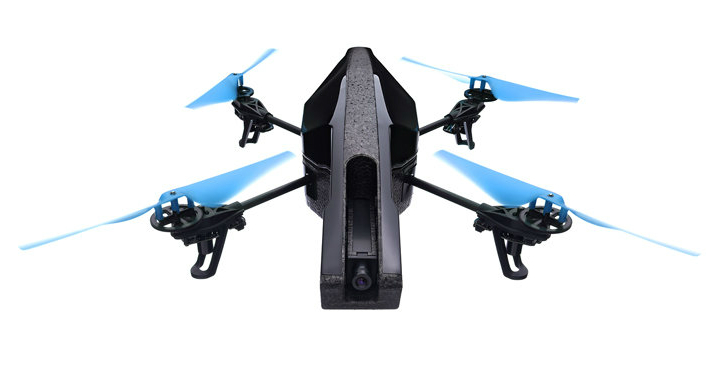
\includegraphics[scale=0.3]{img/parrot_drone.jpg}
	\caption{Plataforma Parrot Ardrone 2.0. Fonte \cite{ardrone}}
	\label{fig:quad}
\end{figure}

\noindent\textbf{Dinâmica de voo}

O objetivo da dinâmica de voo é manter a estabilidade do eixo central do quadricóptero,  controlando os quatro rotores que trabalham de forma independente. Esse processo é considerado complexo e precisa de apoio eletrônico para a execução \cite{Gibiansky2010}. A controladora de voo é responsável por controlar a intensidade das rotações individualmente, de acordo com o movimento preterido. Um dos possíveis controles realizados pela controladora de voo é o PID que será abordado na seção \ref{subsec:PID}.

O quadricóptero é um sistema não linear, fortemente acoplado com seis graus de liberdade, onde três são movimentos lineares ($x$,$y$,$z$) e os outros três angulares ($\phi$,$\theta$,$\psi$). Porém, possui apenas quatro atuadores, sendo considerado então um sistema \textit{underactuated}, com dois movimentos lineares (x,y) dependentes dos movimentos angulares ($\phi$,$\theta$). As forças e momentos atuando no quadricóptero são produzidos pelas hélices ligadas aos rotores. Dois rotores rodam no sentido horário e dois no sentido anti-horário dispostos de forma à balancear o torque total do sistema \cite{Mian2008}. A Figura \ref{fig:diag quad}a mostra a disposição dos motores e suas orientações de funcionamento. Já a Figura \ref{fig:diag quad}b  mostra o diagrama do corpo e os eixos do quadricóptero.

Na Figura \ref{fig:diag quad}b, \textit{l} representa a distância entre cada rotor e o centro, $\phi$, $\theta$ e $\psi$ representam os ângulos de Euler em relação aos eixos x, y e z, chamados de rolagem, afagem e guinada, respectivamente. $T_i$ (i = 1, 2, 3, 4) é a força de empuxo produzida por cada hélice e cada seta circular ao redor de $T_i$ indica o sentido de rotação daquele rotor. O referencial inercial é denotado por $E(X,Y,Z)$ e o referencial do corpo do quadricóptero é denotado por $B(x,y,z)$. 

\begin{figure*}[t]
	\centering
	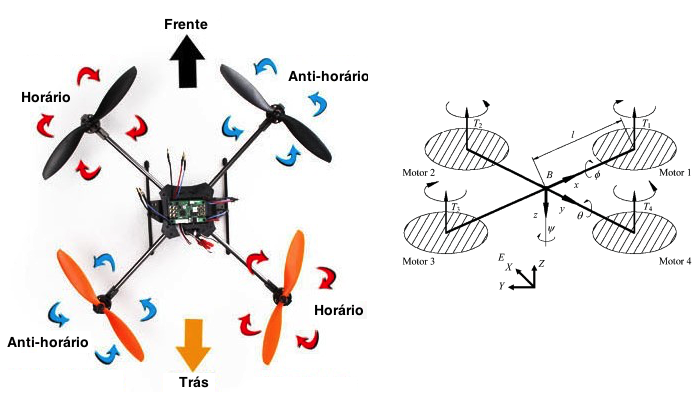
\includegraphics[scale=0.55]{img/diagrama_quadricoptero.png}
	\caption{Estrutura e orientação dos motores (a), as forças e momentos atuando no quadricóptero (b) e os movimentos gerados a partir das variações de velocidades dos motores (c). Fontes \cite{quadblog}, \cite{Mian2008} e \cite{Domingues2009}.}
	\label{fig:diag quad}
\end{figure*}

A Figura \ref{fig:diag quad}c ilustra os movimentos gerados a partir das variações das velocidades dos motores. O aumento ou a diminuição da velocidade dos quatro rotores na mesma proporção irá gerar um movimento vertical (movimentos $a$ e $b$). Quando os motores do par (1,3) operam independentemente e o par (2,4) mantém a mesma velocidade, o ângulo de inclinação do par (1,3), em relação ao eixo $y$ (afagem), poderá ser controlado e, indiretamente, executará um movimento ao longo do eixo $x$ (movimentos $c$ e $d$). Da mesma forma, a operação independente do par de motores (2,4), enquanto (1,3) com velocidade constante, poderá controlar o ângulo de rolagem em relação ao eixo $x$ e um controle indireto do movimento ao longo do eixo $y$ também será realizado (movimentos $e$ e $f$). E, por fim, se ambos os pares possuírem velocidades diferentes, o ângulo de guinada, em relação ao eixo $z$, poderá ser controlado (movimentos $g$ e $h$). Dessa forma, o quadricóptero apresenta seis graus de liberdade e pode ser mover com agilidade em $\mathbb{R}^3$. 

\subsection{Sistemas Embarcados de Navegação}

Navegação inercial é o processo pelo qual se adquirem informações sobre a posição, velocidade e atitude de um veículo com relação a um dado referencial, utilizando informações fornecidas por sensores inerciais tais como acelerômetros e giroscópios. Medindo-se as acelerações e velocidades angulares de um corpo, torna-se possível calcular as mudanças de velocidade, posição e atitude através de sucessivas integrações numéricas \cite{Adalberto2009}.

A unidade de medida inercial, ou IMU, é o componente eletrônico onde são montados os sensores inerciais, sendo três acelerômetros, que fornecem as medidas das componentes da aceleração linear (x,y,z), e três giroscópios, sensores que fornecem as componentes da velocidade angular (por exemplo, arfagem, rolagem e guinada). Já a unidade de processamento é o componente responsável por processar as medidas dos sensores inerciais. As velocidades lineares e as posições são obtidas a partir da integração dos sinais dos acelerômetros, enquanto que a integração dos sinais dos giroscópios fornece a atitude do veículo.  A Figura \ref{fig:imuStrap} ilustra a estrutura de um Sistema de Navegação Inercial acoplado a um veículo, composta por três giroscópios, três acelerômetros (x,y,z) e uma unidade de processamento (CPU) à esquerda e os movimentos gerados no quadricóptero à direita.

\begin{figure*}[b]
	\centering
	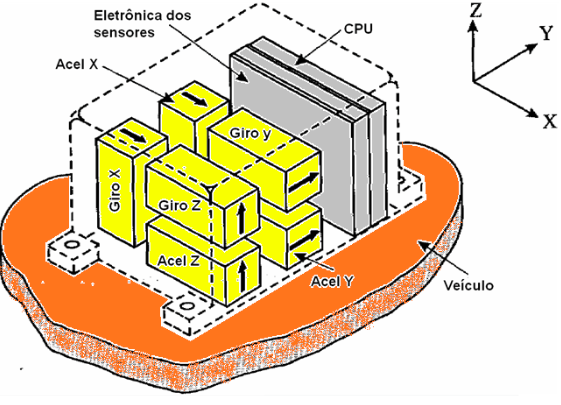
\includegraphics[scale=0.6]{img/imuStrap.png}
	\caption{Estrutura do Sistema de Navegação acoplada ao veículo (esquerda) e os movimentos gerados no quadricóptero (direita). Fonte \cite{Adalberto2009}}
	\label{fig:imuStrap}
\end{figure*}

Magnetômetros podem ser incluídos em IMUs, permitindo uma melhor performance de cálculos de orientação em sistemas AHRS (do inglês, \textit{Attitude Heading Reference System}). Um sistema AHRS é composto de sensores que fornecem a orientação e atitude de uma aeronave. A principal diferença entre uma IMU e um AHRS é a adição de um sistema de processamento embarcado em um AHRS que fornece soluções de atitude e orientação, contra a IMU que apenas fornece os dados do sensor \cite{Angonese2013}.

A Figura \ref{fig:imuVANTIME} demonstra o protótipo de uma IMU desenvolvida para o projeto VANT-IME. No hardware desenvolvido foram utilizados, um acelerômetro que mede a aceleração do veículo e um giroscópio de três eixos para complementar o acelerômetro, obtendo-se assim, informações de velocidade angular em altas frequências, o que se faz necessário para estabilização de aeronaves movendo-se em alta velocidade. Entretanto, devido a erros de deriva dos giroscópios, erros de integração e ao ruído, a utilização de um magnetômetro se faz necessária, pois permite a medição do campo magnético no qual está inserido. As informações de todos os sensores são lidas, filtradas e então processadas para a estimação da atitude da aeronave \cite{Paixao2011}. As Figuras \ref{fig:imuVANTIME}a,  \ref{fig:imuVANTIME}b,  \ref{fig:imuVANTIME}c ilustram as leituras dos sensores inerciais e a Figura \ref{fig:imuVANTIME}d demostra o gráfico resultante após a filtragem e processamento das leituras dos sensores individuais.

\begin{figure*}[b]
	\centering
	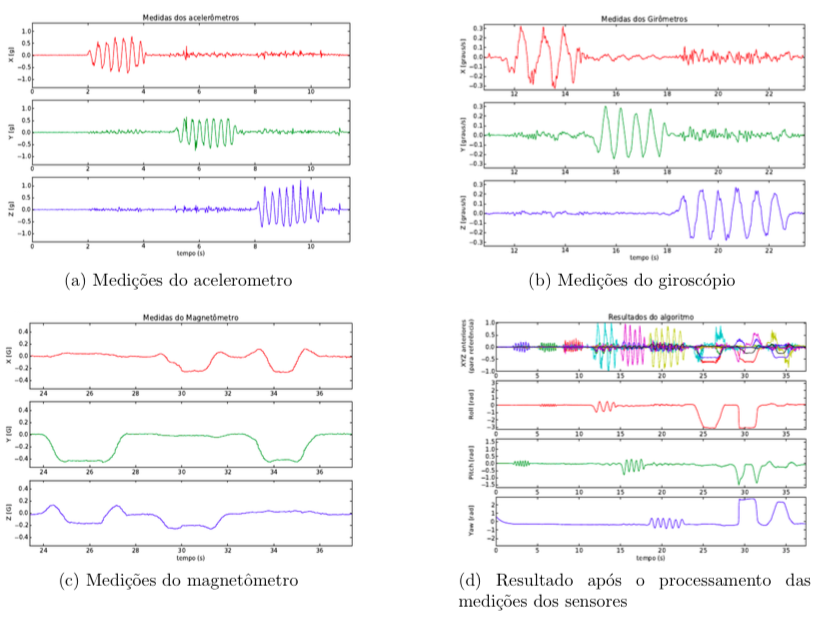
\includegraphics[scale=0.5]{img/imu_VANTIME.png}
	\caption{Gráfico das medições dos sensores inerciais da IMU do VANT-IME. Fonte \cite{Paixao2011}}
	\label{fig:imuVANTIME}
\end{figure*}

\noindent\textbf{Acelerômetros e Giroscópios}

Acelerômetros são sensores que fornecem a medida e a força específica que atua no veículo, que é a resultante das ações da aceleração inercial e da aceleração da gravidade. Portanto, a partir da medida da força específica e do modelo do campo gravitacional da Terra, determina-se a aceleração linear, informação que é integrada para a determinação da velocidade e posição do veículo.

Giroscópios fornecem a medida da velocidade angular. Este dado é utilizado para a determinação da atitude do veículo. Já está na terceira geração. Esta, devido suas características de menor custo e volume, possibilitou sua utilização em grande escala em veículos de pequeno porte. Porém, sua exatidão é menor quando comparado às gerações anteriores. É formado por sensores baseados na tecnologia MEMS (\textit{Micro Electro Mechanical Systems}) que consistem em placas de cerâmicas vibrantes que utilizam Força de Coriolis para medir a taxa independente da aceleração \cite{Adalberto2009}.

\subsection{Controle PID e quadricópteros}

\label{subsec:PID}

Um controle PID é um método comum para controlar robôs e a sua utilidade está na aplicabilidade geral na maioria dos sistemas de controle, principalmente quando o modelo matemático de planta é complexo e não conhecido \cite{Ogata2003}. É um sistema de controle fechado que reage à mudanças no ambiente, que são captadas por sensores, e se baseia na constante sintonia das entradas para obter a saída esperada \cite{Kingdom}.  

O algoritmo de cálculo do controle PID envolve três parâmetros constantes: o valor proporcional (P), o valor integral (I) e o valor derivativo (D) e serão descritos a seguir:

\begin{itemize}
	\item
	Valor proporcional - É tipicamente o erro. Ele é usualmente a distância que o robô deve viajar, ou a temperatura que se queira alcançar. Se o robô está na posição A, mas quer estar na posição B, então o valor proporcional P é $A - B$.
	\item
	Valor integral - É o acúmulo dos erros passados no tempo $t$. Por exemplo, se o robô está continuamente fora da média por uma certa quantidade de tempo, o valor $I$ irá tratar isso. Supondo que em $t_1$ o erro era $A$, em $t_2$ o erro era $B$ e em $t_3$ o erro era $C$. o valor integral I seria $A/t_1 + B/t_2 + C/t_3$.
	\item
	Valor derivativo - É a mudança do erro no tempo $t$. Por exemplo, se o erro era $A$ e, depois do tempo $t$, passou a ser $B$, o valor derivativo $D$ é $(A-B)/t$. Normalmente, o contador de tempo da microcontroladora é utilizado para medir esse tempo. Além disso, $D$ é utilizado para predizer mudanças futuras baseando-se na taxa de mudança atual.
\end{itemize}

A soma ponderada desses três termos é usada para ajustar o processo através de um elemento de controle, como uma válvula ou como o controle da quantidade de energia aplicada ao sistema. O peso é atribuído através de uma constante $K$ denominada ganho e tem o papel de ajustar os valores $P$, $I$ e $D$. Ou seja, cada termo $P$, $I$ e $D$ possui o seu ganho associado e a equação básica de controle é dada pela fórmula \ref{eq:equacaoPID}. 

\begin{equation}
\centering
P*K_p + I*K_i + D*K_d	
\label{eq:equacaoPID}
\end{equation}

A atuação do ganho no desempenho do sistema de controle PID pode ser visualizado na Figura \ref{fig:ganhoPID}, onde a linha azul indica o sinal de referência e as demais linhas indicam diferentes comportamentos com a variação dos ganhos $K_p$, $K_i$ e $K_d$. Um menor tempo de estabilização é normalmente desejável \cite{Kingdom}.  

\begin{figure}[h]
	\centering
	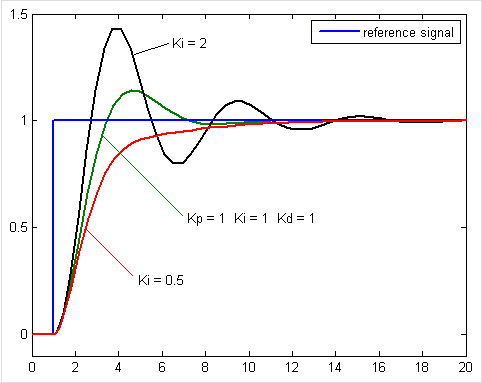
\includegraphics[scale=0.4]{img/ganho_PID.png}
	\caption{Desempenho do sistema para diferentes ganhos $K_p$, $K_i$ e $K_d$. Fonte \cite{Kingdom}}
	\label{fig:ganhoPID}
\end{figure}

\noindent\textbf{PID em quadricópteros}

A maioria dos quadricópteros utilizam PID para estabilização e permitem que o usuário altere os parâmetros para ajustar a performance \cite{Liang}. A Figura \ref{fig:PIDquad} ilustra o esquema de controle PID de um quadricóptero para a estabilização. Basicamente, o \textit{feedback} é obtido através dos sensores do quadricóptero que são avaliados em conjunto com o movimento pretendido pelo piloto através do controle PID e, após, passado ao atuador como comando para os motores. 

\begin{figure}[h]
	\centering
	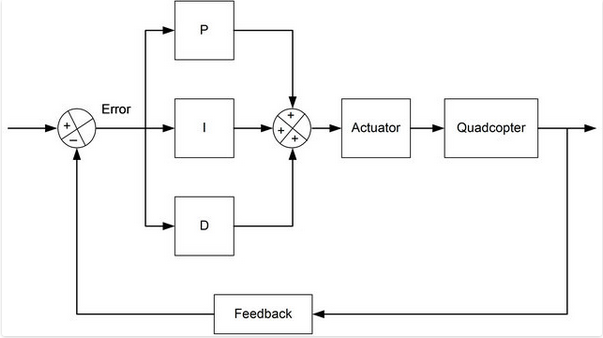
\includegraphics[scale=0.4]{img/PID_quad_geral.png}
	\caption{Controle PID de um quadricóptero. Fonte \cite{Liang}}
	\label{fig:PIDquad}
\end{figure}


Geralmente, segundo \cite{Liang}, existem ao todo três controles PID's, um para cada eixo ($\phi$,$\theta$,$\psi$) e a alteração dos valores dos ganhos ($K_p$, $K_i$ e $K_d$) de cada eixo acarretará em mudanças na reação do quadricóptero quando sujeito a interferências externas. A Figura \ref{fig:PIDaxis} ilustra a estrutura do controle PID de um eixo.

%\begin{itemize}
%\item
%$K_p$ - O quadricóptero pode voar de forma estável somente com esse ganho. Ele determina qual é mais importante, o controle humano ou os valores medidos pelo giroscópio. Quanto maior o coeficiente, mais sensível e reativo ele será para mudanças de ângulos. Se muito pequeno, mais lento e difícil de mantê-lo estável.
%\item
%$K_i$ - Pode aumentar a precisão da posição angular. O tempo de reação à uma alteração do ângulo de inclinação é afetada.
%\item
%$K_d$ - Permite ao quadricóptero alcançar a atitude desejada mais rapidamente. Ele amplifica a ação do usuário. 

%\end{itemize}

\begin{figure}[h]
	\centering
	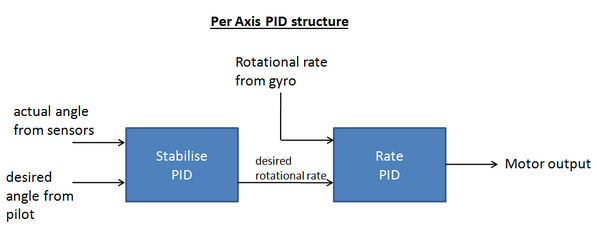
\includegraphics[scale=0.5]{img/PID_quad_axis.png}
	\caption{Controle PID por eixo. Fonte \cite{Liang}}
	\label{fig:PIDaxis}
\end{figure}

% An example of a floating figure using the graphicx package.
% Note that \label must occur AFTER (or within) \caption.
% For figures, \caption should occur after the \includegraphics.
% Note that IEEEtran v1.7 and later has special internal code that
% is designed to preserve the operation of \label within \caption
% even when the captionsoff option is in effect. However, because
% of issues like this, it may be the safest practice to put all your
% \label just after \caption rather than within \caption{}.
%
% Reminder: the "draftcls" or "draftclsnofoot", not "draft", class
% option should be used if it is desired that the figures are to be
% displayed while in draft mode.
%
%\begin{figure}[!t]
%\centering
%\includegraphics[width=2.5in]{myfigure}
% where an .eps filename suffix will be assumed under latex, 
% and a .pdf suffix will be assumed for pdflatex; or what has been declared
% via \DeclareGraphicsExtensions.
%\caption{Simulation Results}
%\label{fig_sim}
%\end{figure}

% Note that IEEE typically puts floats only at the top, even when this
% results in a large percentage of a column being occupied by floats.


% An example of a double column floating figure using two subfigures.
% (The subfig.sty package must be loaded for this to work.)
% The subfigure \label commands are set within each subfloat command, the
% \label for the overall figure must come after \caption.
% \hfil must be used as a separator to get equal spacing.
% The subfigure.sty package works much the same way, except \subfigure is
% used instead of \subfloat.
%
%\begin{figure*}[!t]
%\centerline{\subfloat[Case I]\includegraphics[width=2.5in]{subfigcase1}%
%\label{fig_first_case}}
%\hfil
%\subfloat[Case II]{\includegraphics[width=2.5in]{subfigcase2}%
%\label{fig_second_case}}}
%\caption{Simulation results}
%\label{fig_sim}
%\end{figure*}
%
% Note that often IEEE papers with subfigures do not employ subfigure
% captions (using the optional argument to \subfloat), but instead will
% reference/describe all of them (a), (b), etc., within the main caption.


% An example of a floating table. Note that, for IEEE style tables, the 
% \caption command should come BEFORE the table. Table text will default to
% \footnotesize as IEEE normally uses this smaller font for tables.
% The \label must come after \caption as always.
%
%\begin{table}[!t]
%% increase table row spacing, adjust to taste
%\renewcommand{\arraystretch}{1.3}
% if using array.sty, it might be a good idea to tweak the value of
% \extrarowheight as needed to properly center the text within the cells
%\caption{An Example of a Table}
%\label{table_example}
%\centering
%% Some packages, such as MDW tools, offer better commands for making tables
%% than the plain LaTeX2e tabular which is used here.
%\begin{tabular}{|c||c|}
%\hline
%One & Two\\
%\hline
%Three & Four\\
%\hline
%\end{tabular}
%\end{table}


% Note that IEEE does not put floats in the very first column - or typically
% anywhere on the first page for that matter. Also, in-text middle ("here")
% positioning is not used. Most IEEE journals/conferences use top floats
% exclusively. Note that, LaTeX2e, unlike IEEE journals/conferences, places
% footnotes above bottom floats. This can be corrected via the \fnbelowfloat
% command of the stfloats package.

\section{O Problema: Segurança em voo para quadricóptero}
\label{sec:prob}

O problema a ser tratado consiste em evitar que o quadricóptero se choque, durante sua navegação, através de um método que estima continuamente a trajetória futura do veículo, dada sua dinâmica, seu estado atual, o \textit{input} de controle e a distância para os obstáculos, medida através de sensores ultrassônicos embarcados. Para isso, uma pequena variação no controle será definida baseada em estimativas futuras de colisão. A formulação matemática do problema é descrita a seguir.


%Para isso, torna-se necessário a estimação de sua posição futura, a avaliação de uma possível colisão e a geração de variações de controle a fim de obter um deslocamento seguro. 

\noindent\textbf{Formulação do Problema}

Considerando um quadricóptero como um robô com uma dinâmica não linear genérica em um espaço arbitrário, $\mathcal{X} \subset \mathbb{R}^{n}$ sendo seu espaço de estados e $\mathcal{U} \subset \mathbb{R}^{n}$ o espaço do \textit{input} de controle. Em tempo contínuo, a dinâmica do robô é uma função em $\mathbf{f} \in \mathcal{X} \times \mathcal{U} \times \mathbb{R} \rightarrow \mathbb{R}^{n}$ e é dada pela relação \ref{eq:equacaoDinProb}:

\begin{equation}
\centering
\dot{\mathbf{x}} = \mathbf{f}(\mathbf{x}(t),\mathbf{u}(t),t)  
\label{eq:equacaoDinProb}
\end{equation}

\noindent onde $t$ é o tempo, $\mathbf{x}(t)$ é o estado do robô no tempo $t$ e $\mathbf{u}(t)$ é o \textit{input} de operação no tempo $t$. Consequentemente, dado um estado inicial $\mathbf{x_0} = \mathbf{x}(0)$ e uma constante de \textit{input} de operação $\mathbf{u}$, o estado do robô em um instante $t > 0$ é dado pela relação \ref{eq:equacaoPosProb}:


\begin{equation}
\centering
\mathbf{x} = \mathbf{g}(\mathbf{x},\mathbf{u},t)  
\label{eq:equacaoPosProb}
\end{equation}

\noindent onde $\mathbf{g} \in \mathcal{X} \times \mathcal{U} \times \mathbb{R} \rightarrow \mathcal{X}$ representa a solução da equação diferencial \ref{eq:equacaoDinProb}.

Porém, quando se considera um ambiente repleto de obstáculos, o espaço de estados do robô se restringe à posições não ocupadas por eles. Define-se então $\mathcal{O} \subset \mathbb{R}^3$, como a subárea do espaço $\mathbb{R}^n$ de movimentos possíveis do robô ocupada por obstáculos e as regiões que estão escondidas por eles quando vistas pelo estado corrente do robô. Além disso, $\mathcal{R}(x)$, como a subárea ocupada pelo robô no estado $x \in \mathcal{X}$. Assim, o problema passa a ser definido como identificar a menor variação necessária  $\Delta\mathbf{u} \in \mathcal{U}$ sobre o controle de operação $\mathbf{u}$, dado o atual estado $\mathbf{x}$ do robô, a fim de que se evite uma colisão com algum obstáculo em qualquer momento até se alcançar um período previamente definido $\tau \in \mathbb{R}$ conforme a relação \ref{eq:equacaoProb}:

\begin{equation}
\begin{aligned}
\text{min: }& \Delta\mathbf{u} \\
\text{Sujeito a: }& \forall t \in [0,\tau], \mathcal{R}(\mathbf{g}(\mathbf{x}, \mathbf{u}+\Delta\mathbf{u}, t)) \cap \mathcal{O} = \emptyset
\end{aligned}
\label{eq:equacaoProb}
\end{equation}

%\Delta\mathbf{u^T}T\mathbf{u}

%\noindent onde $T \in R^{m \times m}$ é uma matriz positiva de pesos.

É importante notar que, caso o \textit{input} de operação $\mathbf{u}$ obedeça as restrições da equação \ref{eq:equacaoProb}, ou seja, corresponde a um deslocamento seguro, $\Delta\mathbf{u} = 0$ e nenhuma alteração do controle será realizada.

\section{Metodologia}
\label{sec:meto}

Para resolver este problema, é proposta a seguinte metodologia. Inicialmente, obter medidas de distâncias a partir de sensores ultrassônicos, em tempo real, para detecção de obstáculos. Em seguida, confrontá-los com os dados, já filtrados, da atitude do quadricóptero obtidos da IMU para identificar colisões iminentes em uma janela de tempo pré-determinada. Em caso positivo, interceptar o comportamento gerando uma pequena mudança de comando que seja suficiente para evitar uma colisão naquela janela de tempo.

Para facilitar o entendimento, o método foi dividido em etapas que serão  descritas a seguir, juntamente com os componentes e software necessário e a estratégia de sua implementação.

\subsection{Etapas}

\label{subsec:etapas}

A Figura \ref{fig:etapasMetodo} ilustra as etapas envolvidas, onde cada cor representa um tipo de atuação e as setas indicam suas dependências. Em azul estão os responsáveis pela aquisição dos dados necessários: sensores ultrassônicos, os comandos de controle e a os sensores da IMU. Em verde, estão os processos de tratamento dos dados a fim de se obter medidas confiáveis para os módulos. Já em amarelo estão os módulos centrais para detecção de obstáculos e identificação de colisões. Por fim, em vermelho, está o controle de atitude, processo integrante da controladora de voo, que receberá comandos e os transformarão em ações do quadricóptero.   

\begin{figure}[h]
	\centering
	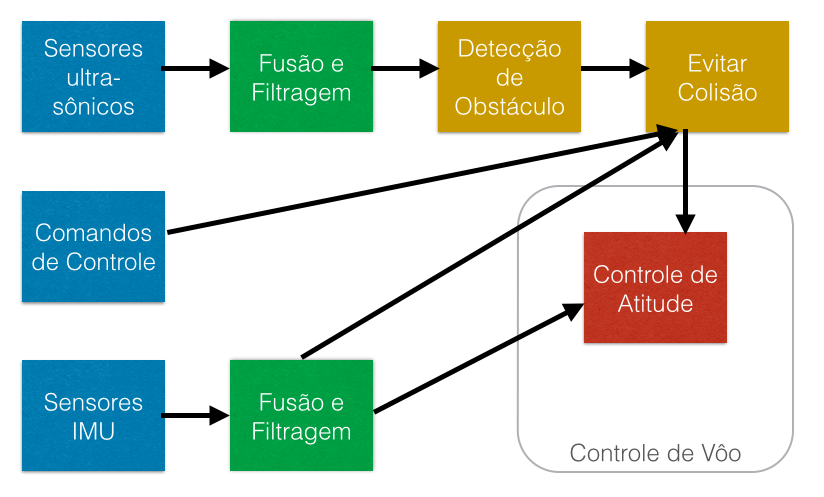
\includegraphics[scale=0.3]{img/etapasMetodo.png}
	\caption{Etapas do método}
	\label{fig:etapasMetodo}
\end{figure}

Em seguida, as etapas e uma breve descrição dos passos necessários para galgá-las no trabalho proposto:

\noindent\textbf{Sensores ultrassônicos} 
\begin{itemize}
	\item
	Definir o modelo e a quantidade de sensores ultrassônicos a serem utilizados e como dispô-los de forma a obter uma região de cobertura adequada.  
\end{itemize}

\noindent\textbf{Fusão e Filtragem dos Sensores} 
\begin{itemize}
	\item
	Definir e estudar o método que será utilizado para fusão dos sensores ultrassônicos.
\end{itemize}

\noindent\textbf{Comandos e Controle} 
\begin{itemize}
	\item
	Estudar o \textit{software development kit}, a partir daqui, chamado de SDK, de controle da plataforma de voo.  
\end{itemize}

\noindent\textbf{Sensores IMU} 
\begin{itemize}
	\item
	Verificar como obter os dados da IMU da plataforma de voo através de seu SDK.
\end{itemize}

\noindent\textbf{Fusão e Filtragem da IMU} 
\begin{itemize}
	\item
	Estudar a utilização dos dados já filtrados pela plataforma de voo.  
\end{itemize}

\noindent\textbf{Detecção de Obstáculos} 
\begin{itemize}
	\item
	Estudar e implementar o mapeamento dos obstáculos visíveis a partir das medidas obtidas dos sensores em um dado momento.  
\end{itemize}

\noindent\textbf{Identificação de Colisão} 
\begin{itemize}
	\item
	Estudar e implementar o método para controle de colisão janela dinâmica que será utilizado para detecção de colisão com os obstáculos mapeados. 
	\item
	Estudar a dinâmica de voo da plataforma de voo e implementar a extrapolação de sua posição em um dado período de tempo.  
\end{itemize}

\noindent\textbf{Controle de Atitude} 
\begin{itemize}
	\item
	Verificar o padrão de troca de comandos entre os comandos de controle e a controladora de voo para a implementação através do SDK.  
\end{itemize}

\subsection{Componentes necessários}

\label{subsec:hardware}

Para realização deste trabalho, é necessária a utilização de uma plataforma de voo (quadricóptero) que aceite \textit{input} de controle gerado por computador, através de uma interface de comunicação, e que possua SDK de código aberto para facilitar o desenvolvimento de algoritmos para seu controle.

Embarcado na plataforma, além dos sensores ultrassônicos, será necessário um \textit{computer on module}. Ele será responsável por colher e filtrar os dados dos sensores ultrassônicos, rodar o algoritmo para detecção de obstáculos, obter os comandos de controle, identificar possíveis colisões e enviar comando para o controle de atitude. Para isso, será utilizado o \textit{computer on module} Raspberry PI. 

\subsection{Software necessário}

\label{subsec:software}

Inicialmente, o trabalho será desenvolvido em um ambiente simulado \textit{hardware-in-the-loop} em MATLAB Simulink, para então ser testado na plataforma de voo. Para simular o quadricóptero, será utilizado um kit de desenvolvimento para quadricópteros do Matlab Simulink, que permite a simulação e o controle em tempo real da plataforma. Já a obtenção de dados dos sensores e o desenvolvimento dos algoritmos serão realizados com o apoio do \textit{Raspberry Pi Support from MATLAB}, que provê acesso aos periféricos através do Raspberry Pi, permitindo adquirir dados dos sensores conectados em tempo real.

\subsection{Estratégia de implementação}

A implementação da solução consiste basicamente em duas fases do cronograma desta proposta que será ilustrado na seção \ref{sec:crono}: Fase de Simulação e Fase de testes com a Plataforma. Baseado nas etapas descritas na seção \ref{subsec:etapas} e nos itens de hardware e software descritos nas seções \ref{subsec:hardware} e \ref{subsec:software}, a estratégia de implementação pode ser visualizada na Figura \ref{fig:Fluxo}. Em paralelo, o ambiente para simulação será montado enquanto as aquisições necessárias serão realizadas. Após, a implementação da solução será executada de forma incremental, com o primeiro ciclo utilizando apenas um sensor ultrassônico para validação dos algoritmos de detecção de obstáculo e identificação de colisão. Em seguida, serão adicionado outros sensores na solução em um segundo ciclo. Por fim, a plataforma então será utilizada, para realização de testes em campo e o embarque da solução completa.

\begin{figure}[h]
	\centering
	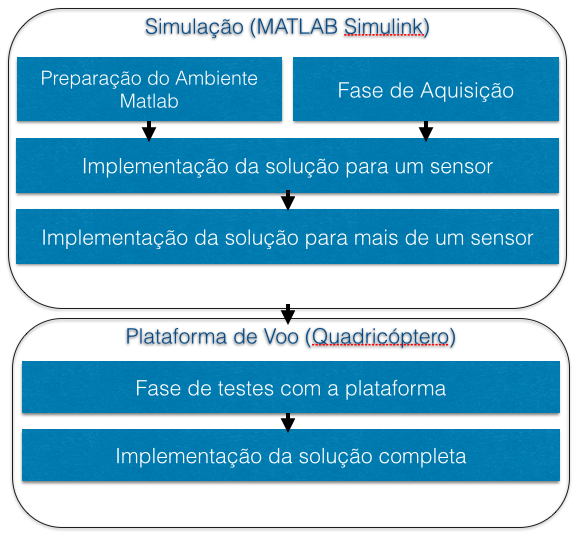
\includegraphics[scale=0.4]{img/fluxo.png}
	\caption{Estratégia de implementação}
	\label{fig:Fluxo}
\end{figure}

\section{Resultados esperados}
\label{sec:resultados}
Para avaliação do método, foram estipuladas três missões que o quadricóptero precisa ser capaz de realizar. Em todas, ele deverá evitar a colisão, mantendo uma distância segura dos obstáculos. Cada missão avalia o método em diferentes situações e estão descritas a seguir.

\noindent\textbf{Missão 1: Manter sua posição enquanto estabilizado e nenhuma saída}

O quadricóptero será estabilizado e cercado, não tendo caminho possível de ser realizado enquanto o piloto executa comandos de controle. O \textit{input} do controle será ignorado, ou seja, qualquer comando realizado pelo piloto será desprezado e a plataforma manterá sua posição. Um esboço da situação pode ser visualizado na Figura \ref{fig:missao1}. Esta missão irá avaliar se o método consegue evitar os obstáculos em todas direções $(x,y)$.

\begin{figure}[h]
	\centering
	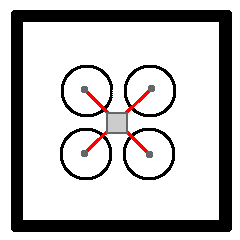
\includegraphics[scale=0.5]{img/missao1.png}
	\caption{Missão 1. Veículo cercado e estabilizado}
	\label{fig:missao1}
\end{figure}  

\noindent\textbf{Missão 2: Desviar de um obstáculo estático a frente}

Nesta missão, o quadricóptero será conduzido a uma velocidade de aproximadamente $2m/s$ através de uma trajetória retilínea em um ambiente \textit{indoor} enquanto depara-se com um obstáculo a frente. Ele irá realizar um desvio pela lateral do obstáculo. Será escolhido o lado que exija o menor desvio possível (Figura \ref{fig:missao2}). Esta missão irá avaliar se o método consegue desviar a trajetória do quadricóptero, perante um obstáculo, quando em movimento.

\begin{figure}[h]
	\centering
	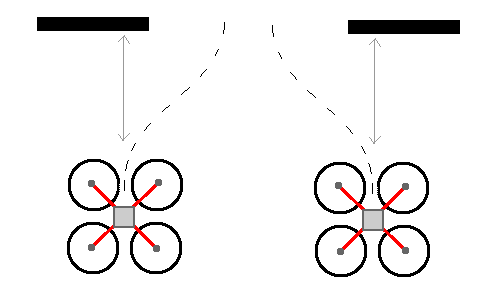
\includegraphics[scale=0.5]{img/missao2.png}
	\caption{Missão 2: Veículo em movimento com obstáculo a frente. Um desvio à direita (esquerda) e um desvio à esquerda (direita)}
	\label{fig:missao2}
\end{figure}  

\noindent\textbf{Missão 3: Realizar uma trajetória segura num ambiente com vários obstáculos} 

Por fim, o quadricóptero será conduzido a uma velocidade de aproximadamente $2m/s$ por um trajeto completo, com diversos obstáculos em posições variadas, e ele deverá ser capaz de terminá-lo sem colisões. O objetivo desta missão é avaliar a eficácia e o benefício do método simulando a condução de um quadricóptero num ambiente complexo de difícil pilotagem. A Figura \ref{fig:missao3} ilustra o mapa do ambiente a ser utilizado com as setas indicando o início e o fim do trajeto.


\begin{figure}[h]
	\centering
	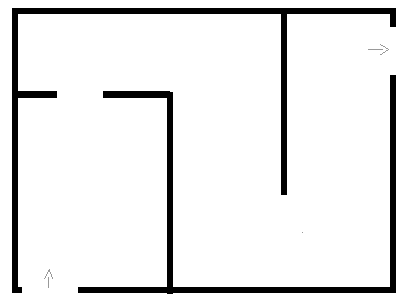
\includegraphics[scale=0.4]{img/missao3.png}
	\caption{Missão 3: Trajeto completo num ambiente com obstáculos}
	\label{fig:missao3}
\end{figure}  


\section{Conclusion}
\label{conclusao}

O advento da utilização dos VANT's, mais especificamente os quadricópteros, em ambientes restritos, trazem a tona a necessidade de controlar o desvio de obstáculo de forma automática. Este é um tema que tem merecido atenção na área de robótica e nossa proposta visa explorá-lo com medições de sensores em tempo real, auxiliando o controle do veículo. Com esse enfoque, nossa proposta é viável e poderá ser utilizada em uma variedade de aplicações na área de defesa.  Além disso, a solução, uma vez construída, será o módulo de desvio de obstáculos da plataforma VANT-IME, que está em fase de concepção no Laboratório RoboIME.




% conference papers do not normally have an appendix


% use section* for acknowledgement
\section*{Acknowledgment}


The authors would like to thank...





% trigger a \newpage just before the given reference
% number - used to balance the columns on the last page
% adjust value as needed - may need to be readjusted if
% the document is modified later
%\IEEEtriggeratref{8}
% The "triggered" command can be changed if desired:
%\IEEEtriggercmd{\enlargethispage{-5in}}

% references section

% can use a bibliography generated by BibTeX as a .bbl file
% BibTeX documentation can be easily obtained at:
% http://www.ctan.org/tex-archive/biblio/bibtex/contrib/doc/
% The IEEEtran BibTeX style support page is at:
% http://www.michaelshell.org/tex/ieeetran/bibtex/
\bibliographystyle{IEEEtran}


%\bibliographystyle{abbrv}

\bibliography{Dissertacao} 
% argument is your BibTeX string definitions and bibliography database(s)
%\bibliography{IEEEabrv,../bib/paper}
%
% <OR> manually copy in the resultant .bbl file
% set second argument of \begin to the number of references
% (used to reserve space for the reference number labels box)



% that's all folks
\end{document}


